\section{Miscellaneous 3D Printed Parts}
For this project, extensive use was made of the 3D printer available in the innovation lab at T5.
In order to improve the presentation of WTR, as many loose parts as possible have been slotted into custom designed sleeves or boxes, clipped into place on the frame.
Some parts have been screwed into the wood, such as the 4 Raspberry Pi's, which now have increased accessibility.
Any measurements used were either looked up in the relevant data sheets, or measured using a caliper with a +-0.10mm inaccuracy.

\subsection{Boxes and Containers}
\subsubsection{IMU container}
Since the IMU needs to be away from Iron as far as possible, the decision was made to clip it to the top of the TV screen.

\begin{figure}[H]
\centering
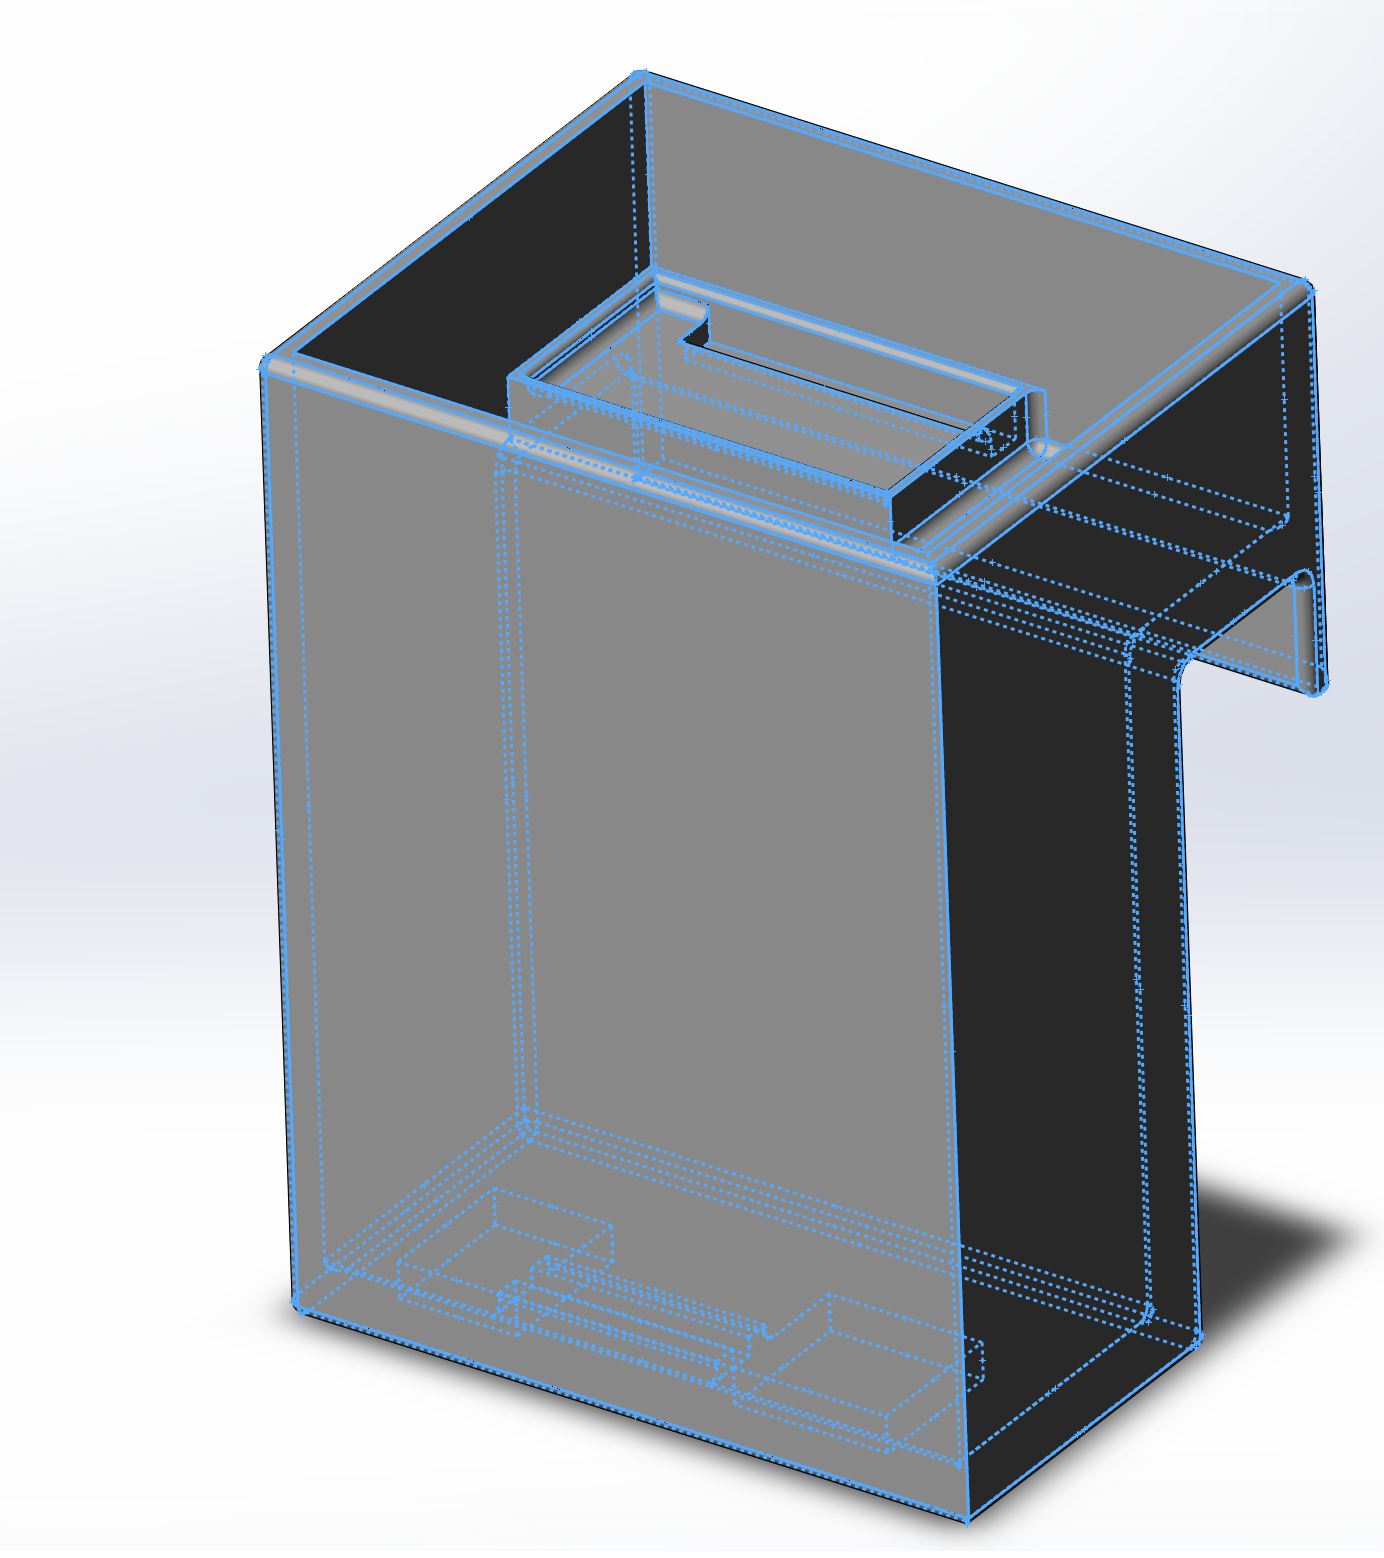
\includegraphics[width=12cm]{/3ddesign/imubak.png}
\caption{A partially wireframed model of the casing for the IMU and an Arduino}
\label{fig::IMUB}
\end{figure}

As shown in figure \ref{fig::IMUB}, the case has a hooked top, which allows it to hang to from the top of the screen.
It also has a slot for an Arduino, kept in place using the USB port, as well as the power jack.
In addition, a small slot has been made at the bottom for the PCB section to fit into.

The IMU is contained in a small rectangular section at the top, with a smaller rectangle cut out to allow the pins to slot in neatly.
A lid can be placed on top of the box, to allow it to be closed off and less likely to be interfered with.

\subsubsection{Sonar Arduino container}
The container for the arduino that pings all the HC-SR04 sensors can be found near the sensor node Pi, clipped onto the side of WTR.
It is a small box with a few rectangles cut out of the lid to allow wire to pass through, from the arduino to the sensors.

\begin{figure}[H]
\centering
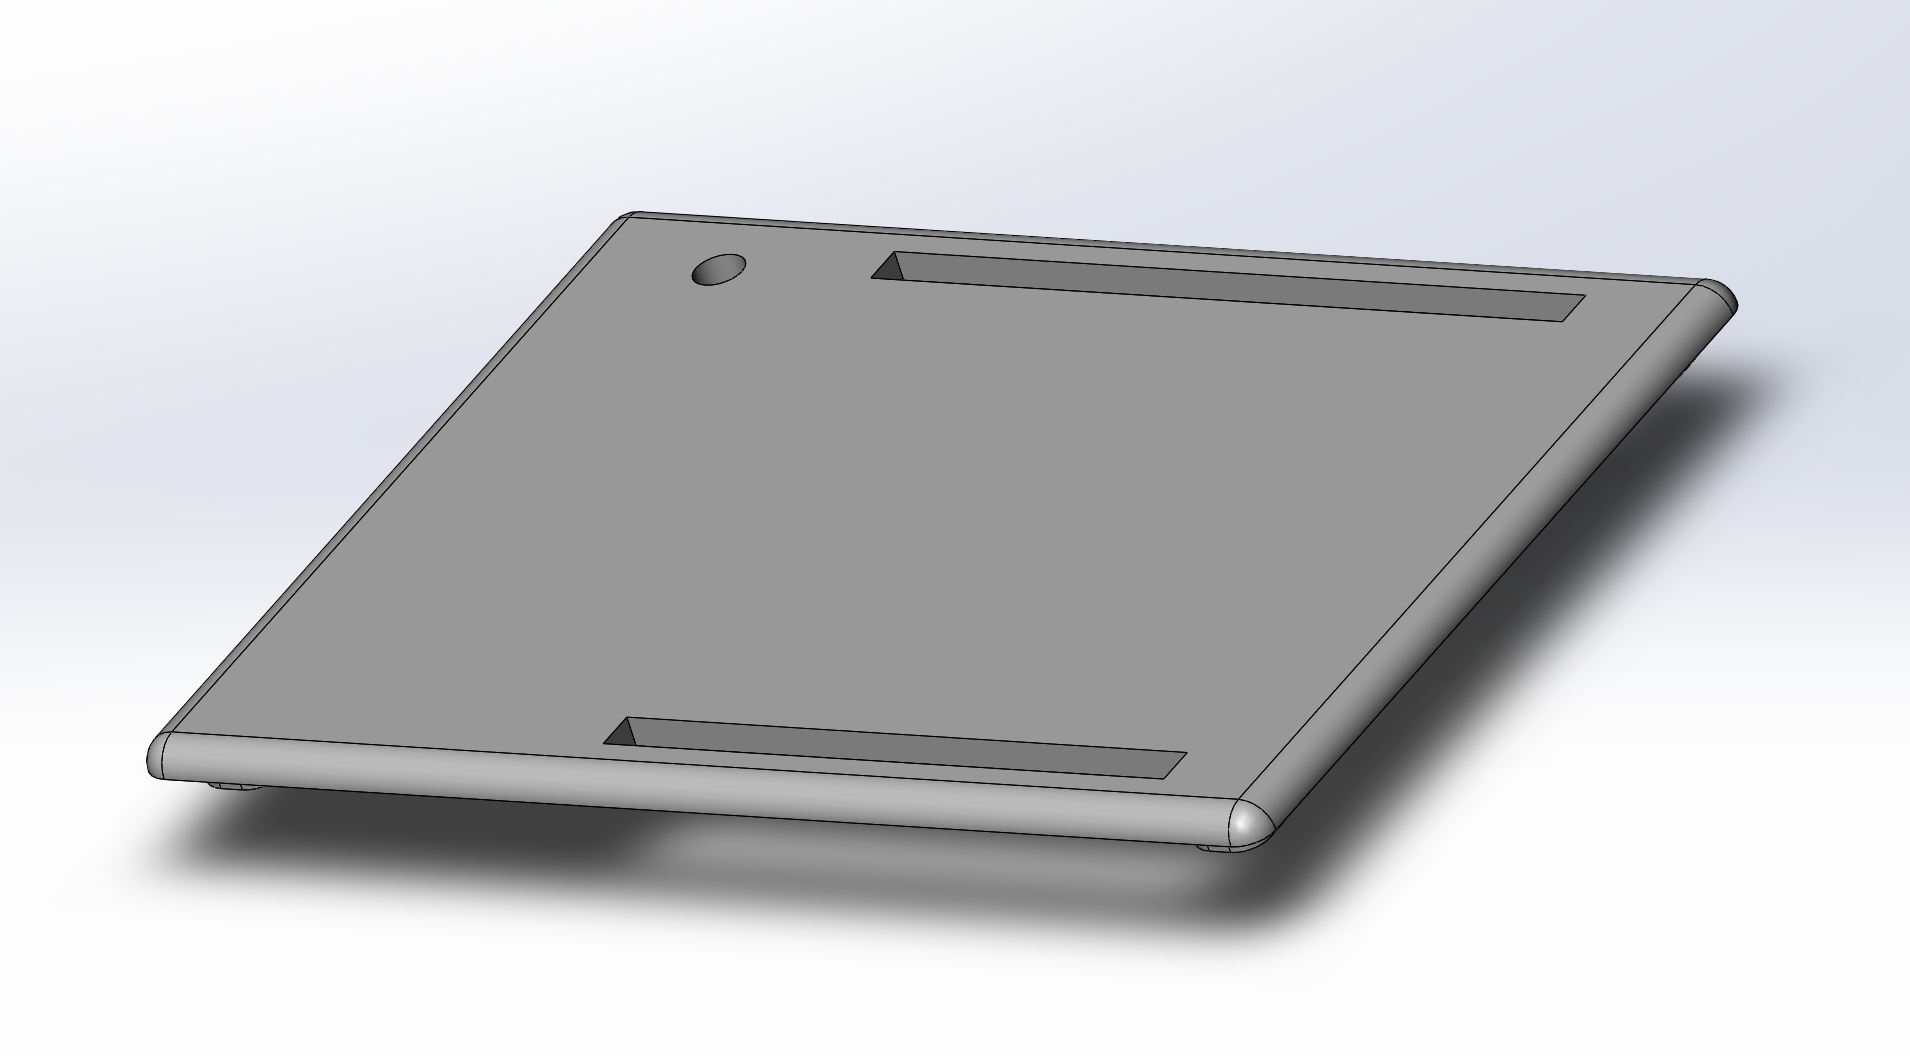
\includegraphics[width=10cm]{/3ddesign/ardlidson.png}
\caption{The lid of the arduino container}
\label{fig::ardLidSon}
\end{figure}

\begin{figure}[H]
\centering
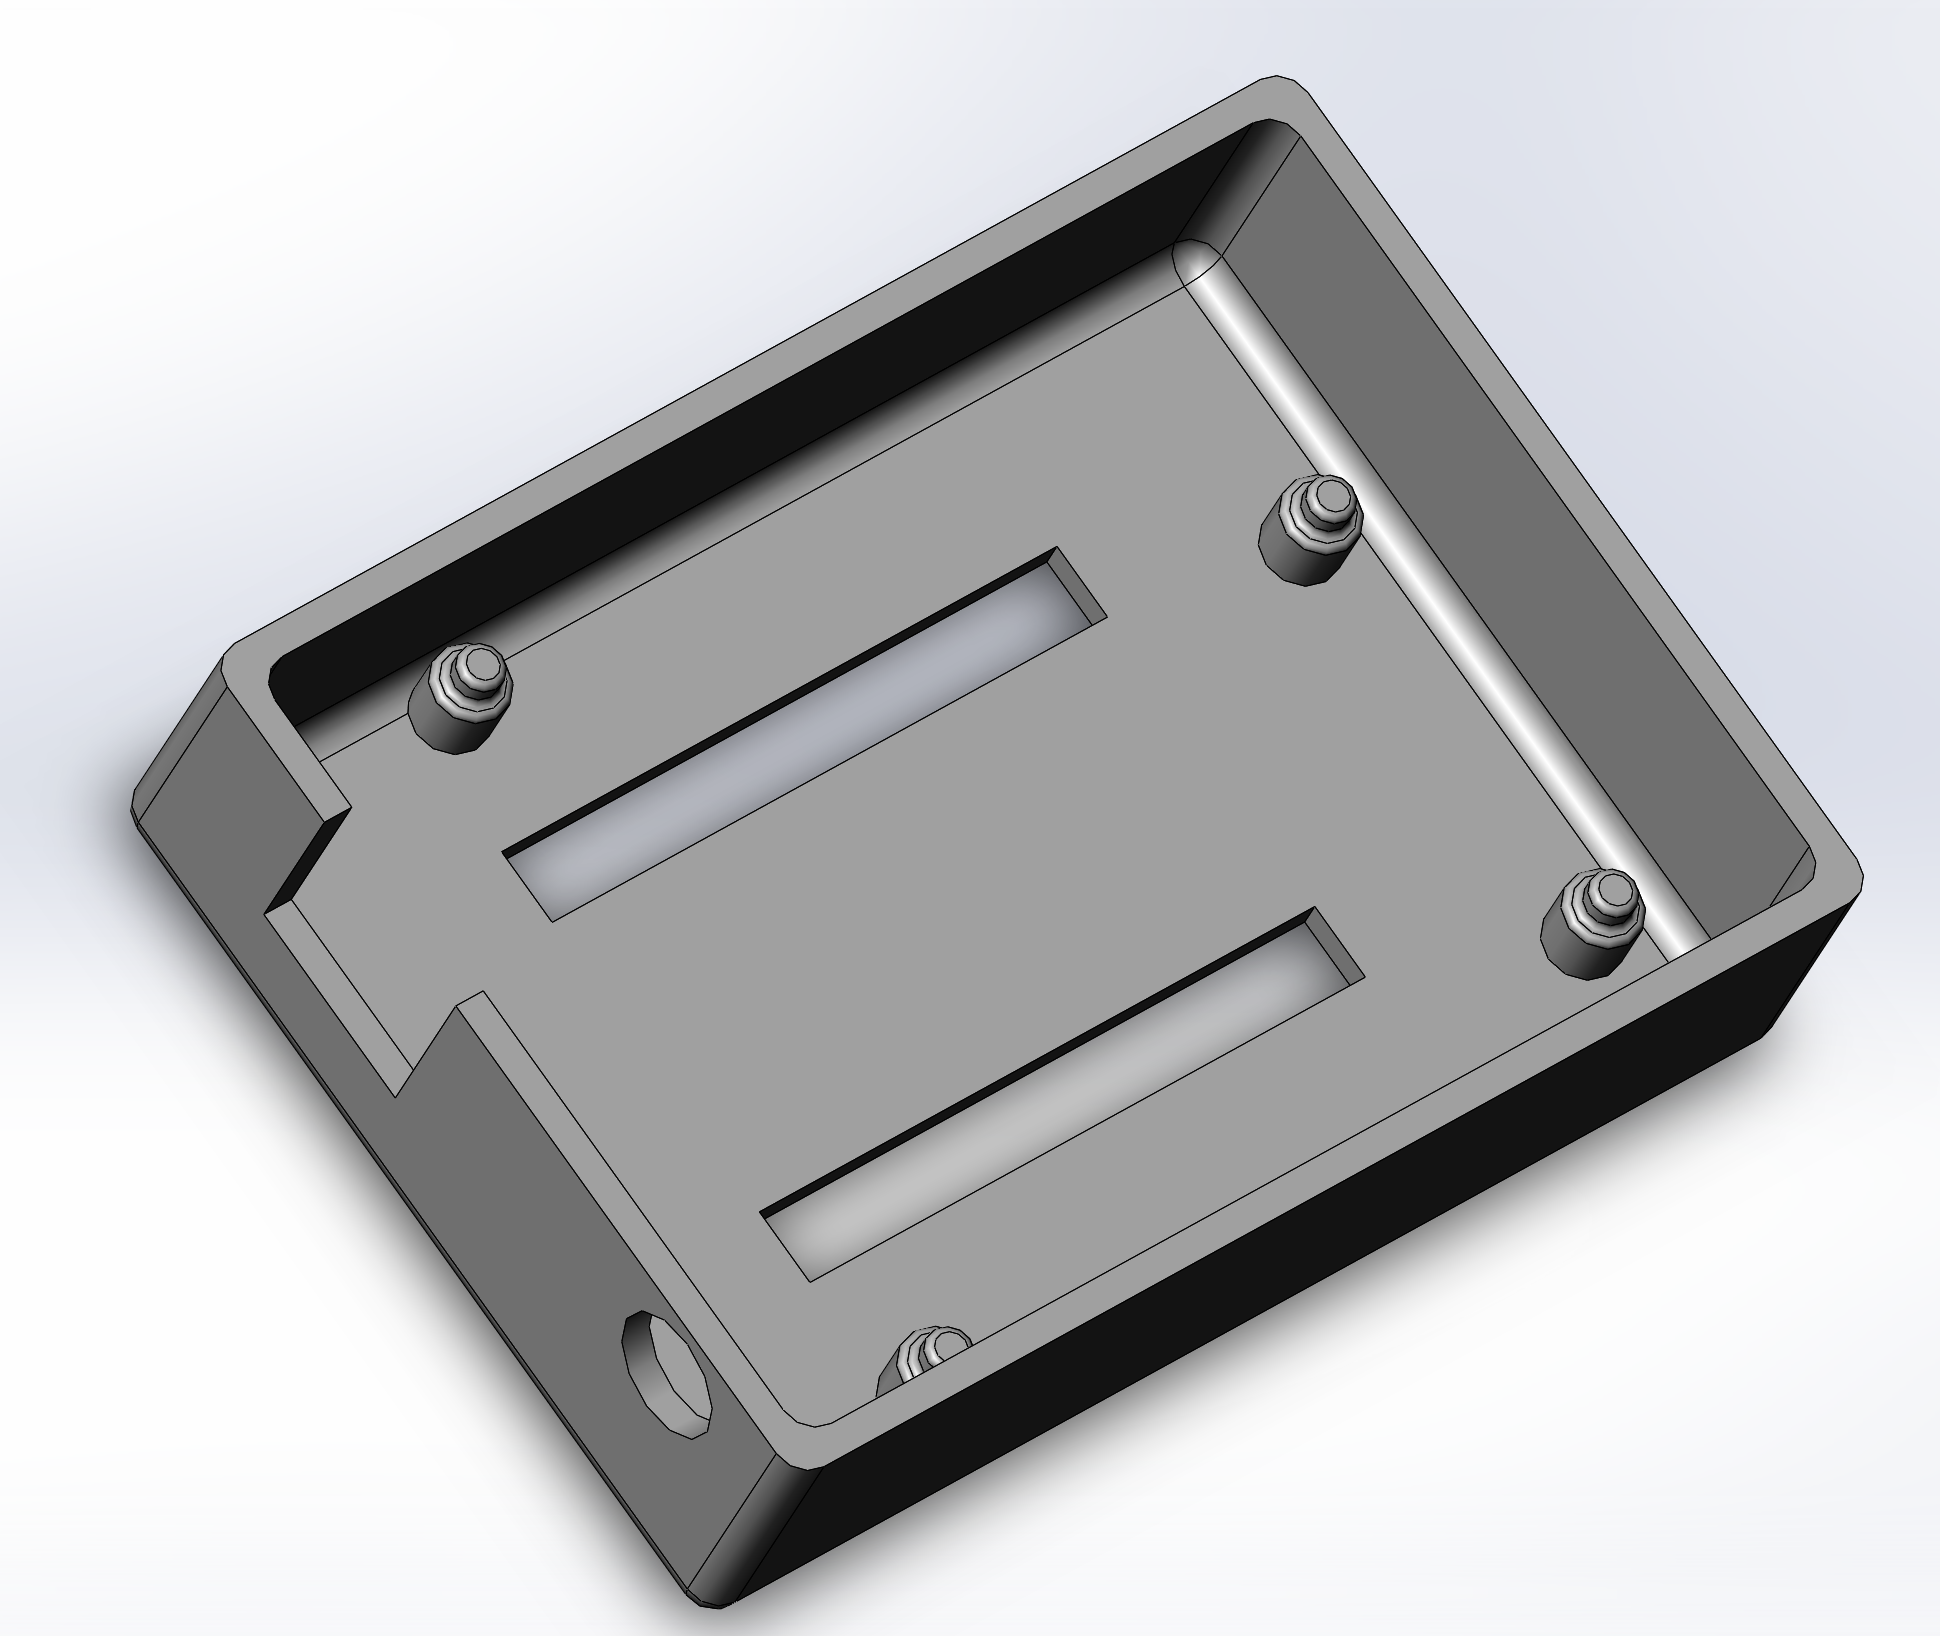
\includegraphics[width=12cm]{/3ddesign/ardconson.png}
\caption{The container of the arduino that pings the HC-SR04 sensors}
\label{fig::ardConSon}
\end{figure}

All of the arduino containers, unless otherwise specified, are attached to WTR via two slots in the bottom of the container and a clamp which fits around the metal beams the frame consists of.

\begin{figure}[H]
\centering
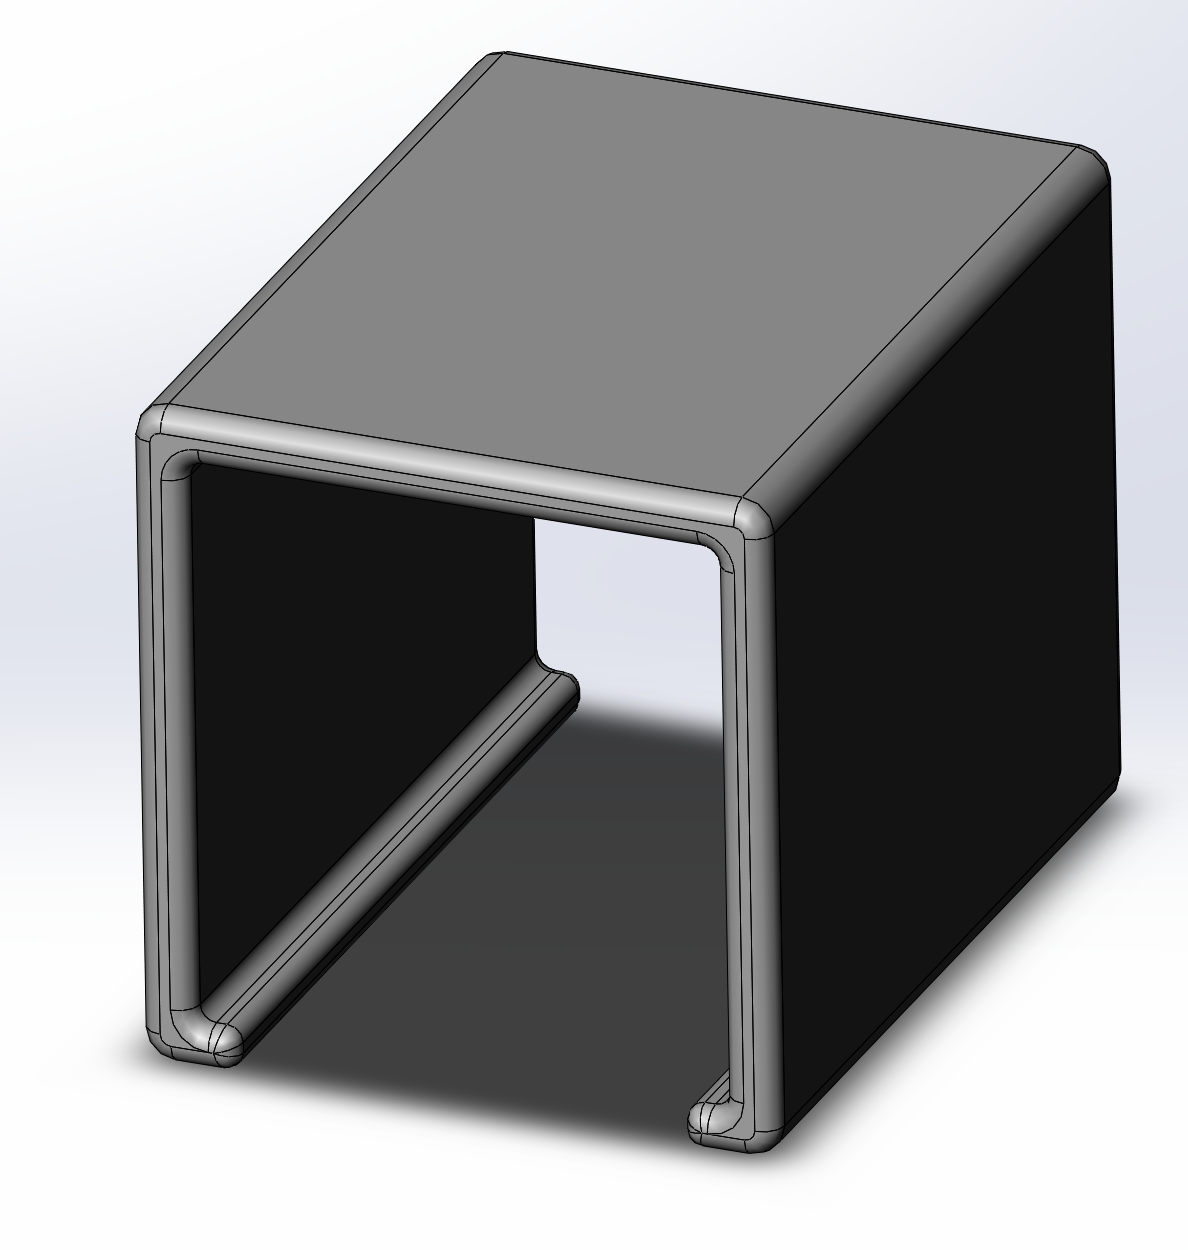
\includegraphics[width = 12cm]{/3ddesign/clamp.png}
\caption{the clamp that fits around a 25mm steel beam, with some room to spare to accommodate the containers}
\label{fig::clamp}
\end{figure}

\subsection{Emergency Stop}
The emergency stop is mounted via an open-topped box, with pins at the bottom that taper inward slightly.
This is to ensure a snug fit, which prevents the emergency stop from being removed accidentally.
Previously, it was glued to the frame via hot glue.
This is an obvious security risk, since hot glue does not adhere well to metal.

\begin{figure}[H]
\centering
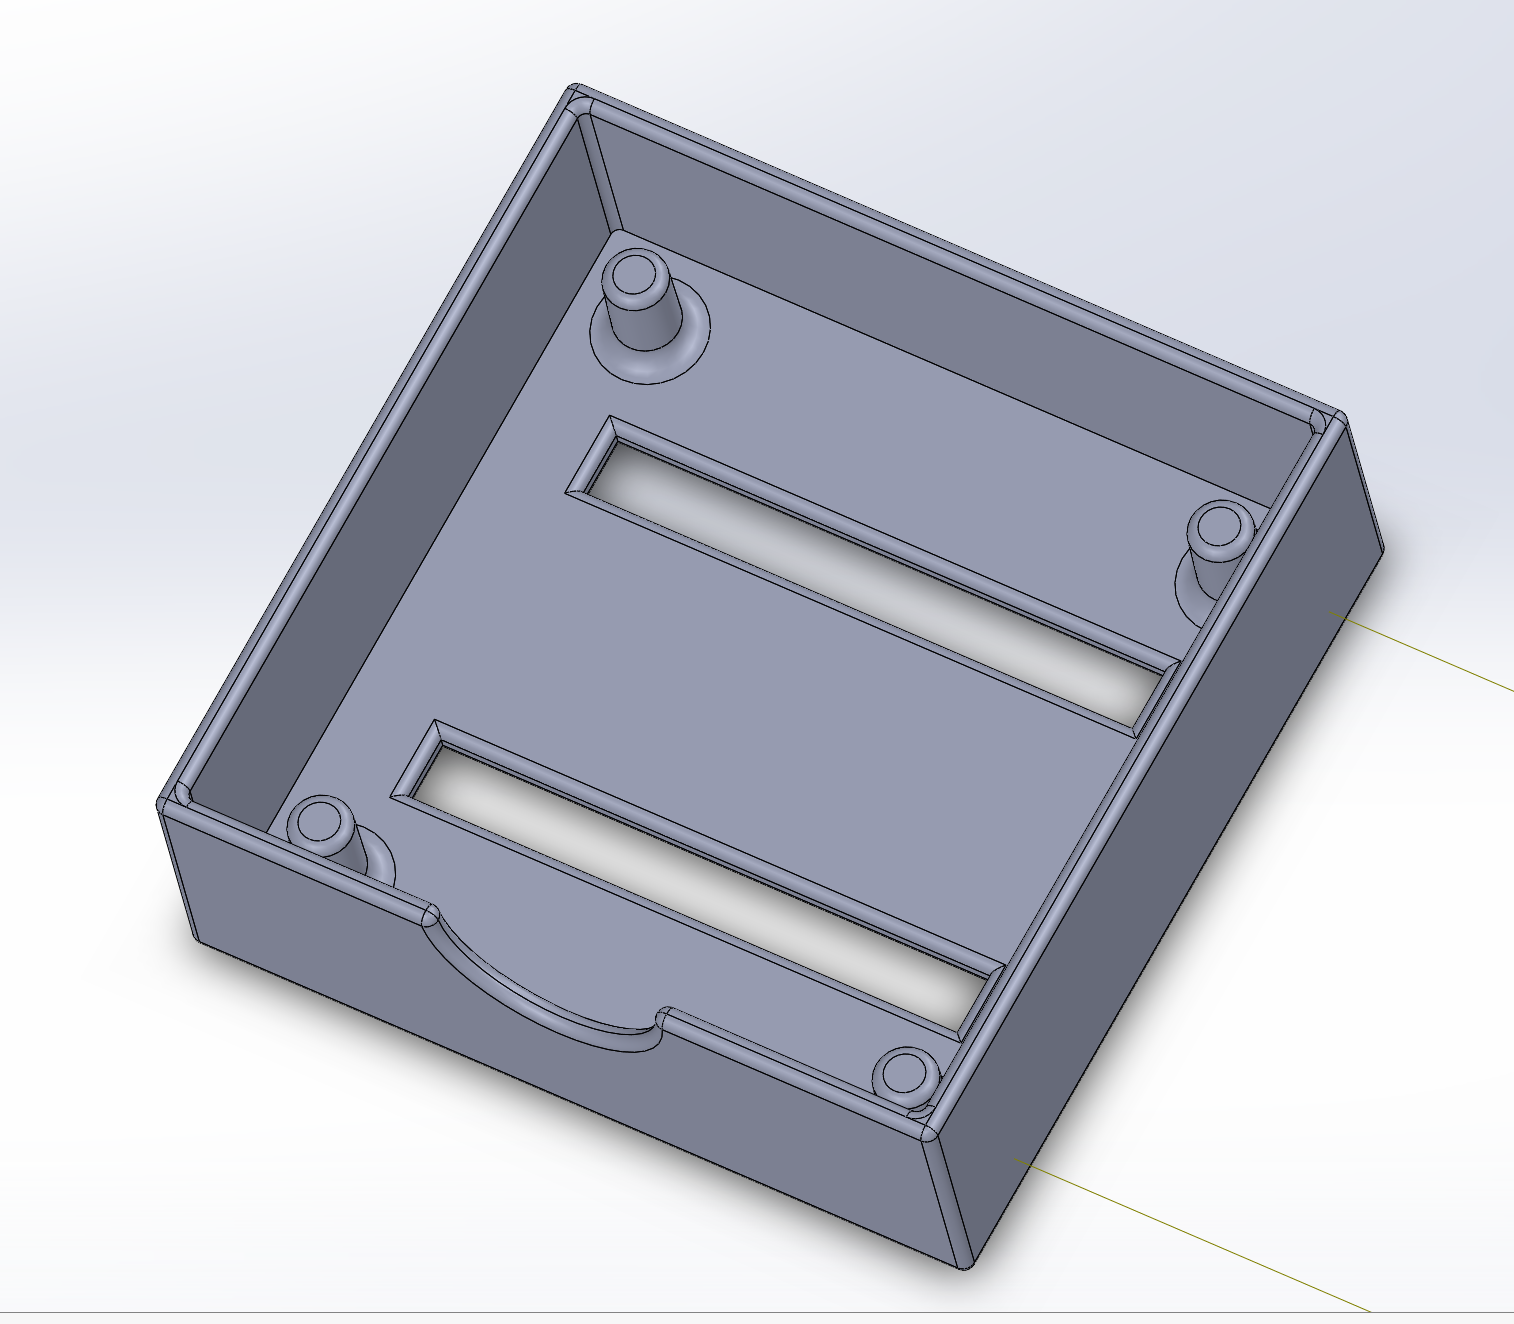
\includegraphics[width=12cm]{/3ddesign/emergency.png}
\caption{The container for the emergency stop button}
\label{fig::ESB}
\end{figure}

The container is attached to the frame using a clamp shown in figure \ref{fig::clamp}.

\subsection{PS3 Controller Hook}
The PS3 DualShock controller was previously simply left wherever space was available.
This was not presentable, and contributed to the clutter of wires.
Instead, a hook has been designed that incorporates the cable that connects the controller to the PC, and prevents it from falling off or causing clutter.

\begin{figure}[H]
\centering
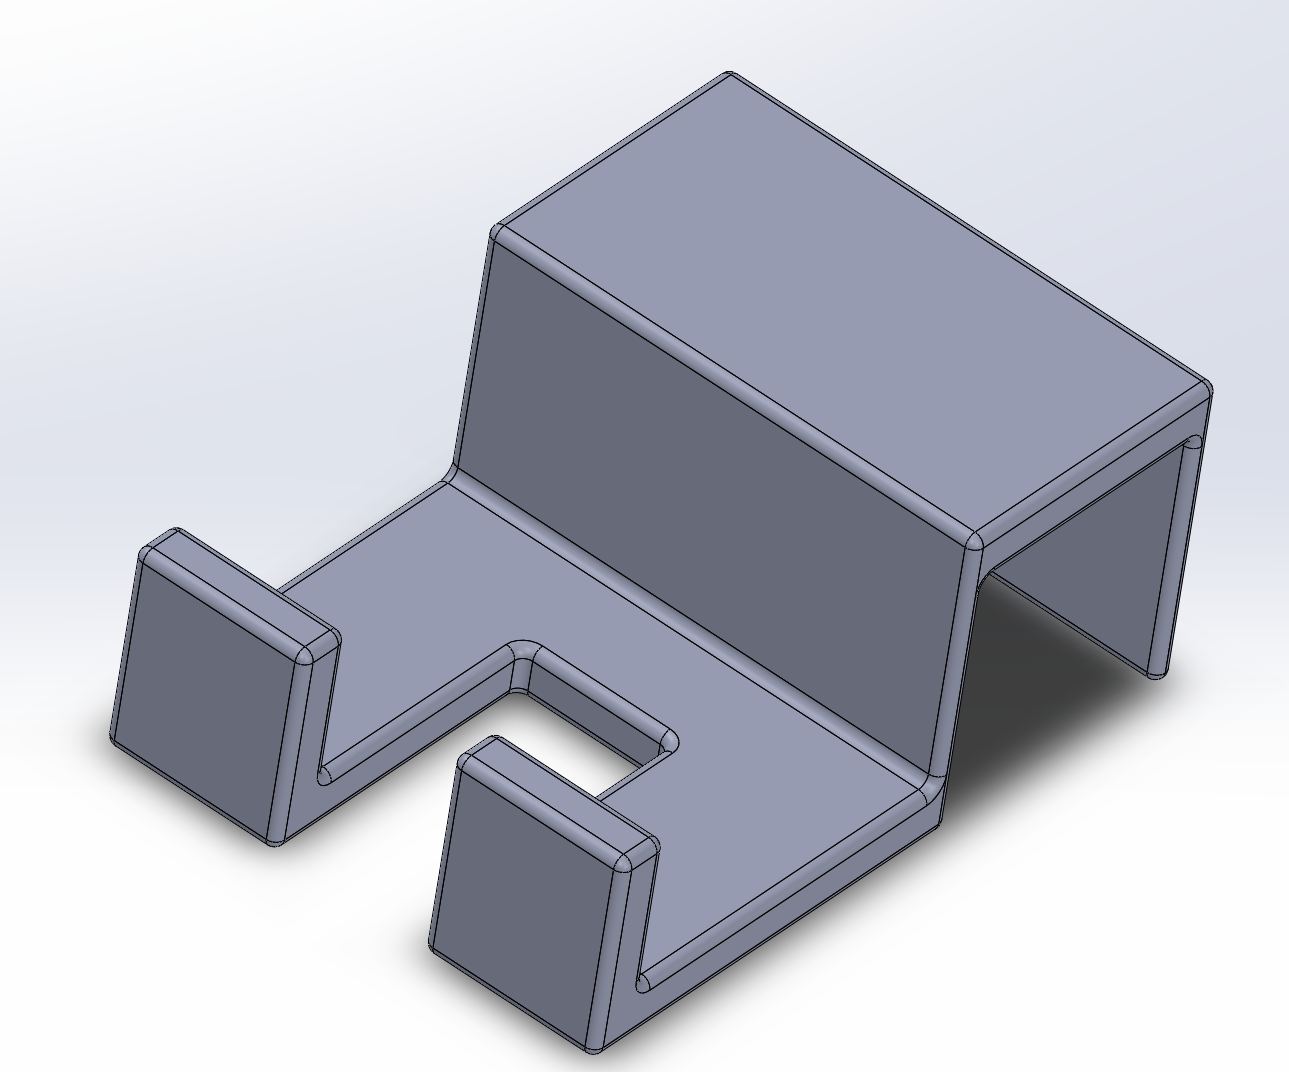
\includegraphics[width=12cm]{/3ddesign/ps3mount.png}
\caption{A mount for the PS3 controller}
\label{fig::PS3}
\end{figure}

This clamps around a metal beam much like the clamp shown in figure \ref{fig::clamp}.
It can be found above the laptop, in the middle of the frame.

\subsection{Coverings}
WTR has already claimed 2 fabric-based casualties.
2 sets of jeans have already had a hole torn in them due to sharp metal protrusions extending from the frame of WTR.
In order to prevent further incidents, some caps have been designed and printed that cover the sharp bits, without permanently removing the mounting opportunities for the white cover that can also be found in the innovation lab on T5.


\begin{figure}[H]
\centering
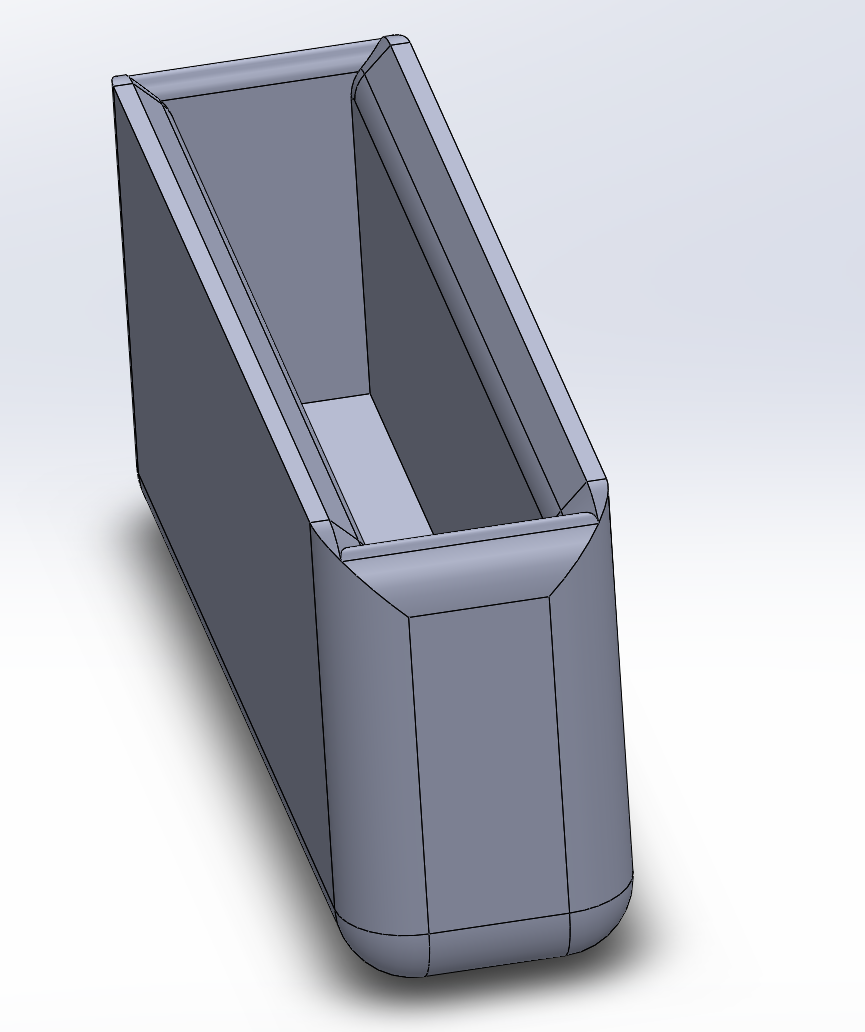
\includegraphics[width=12cm]{/3ddesign/covers.png}
\caption{The caps that cover the sharp protrusions}
\label{fig::CAP}
\end{figure}

\subsection{Fan Covering}
A cover has been designed and printed to cover the cooling fan that keeps the voltage transformers at a stable temperature.
Previously, this fan was exposed.
This is obviously a safety hazard if WTR is to be driving in public.
The cover has large enough gaps to allow airflow, but small enough to prevent accidentally touching the moving fan blades.

\begin{figure}[H]
\centering
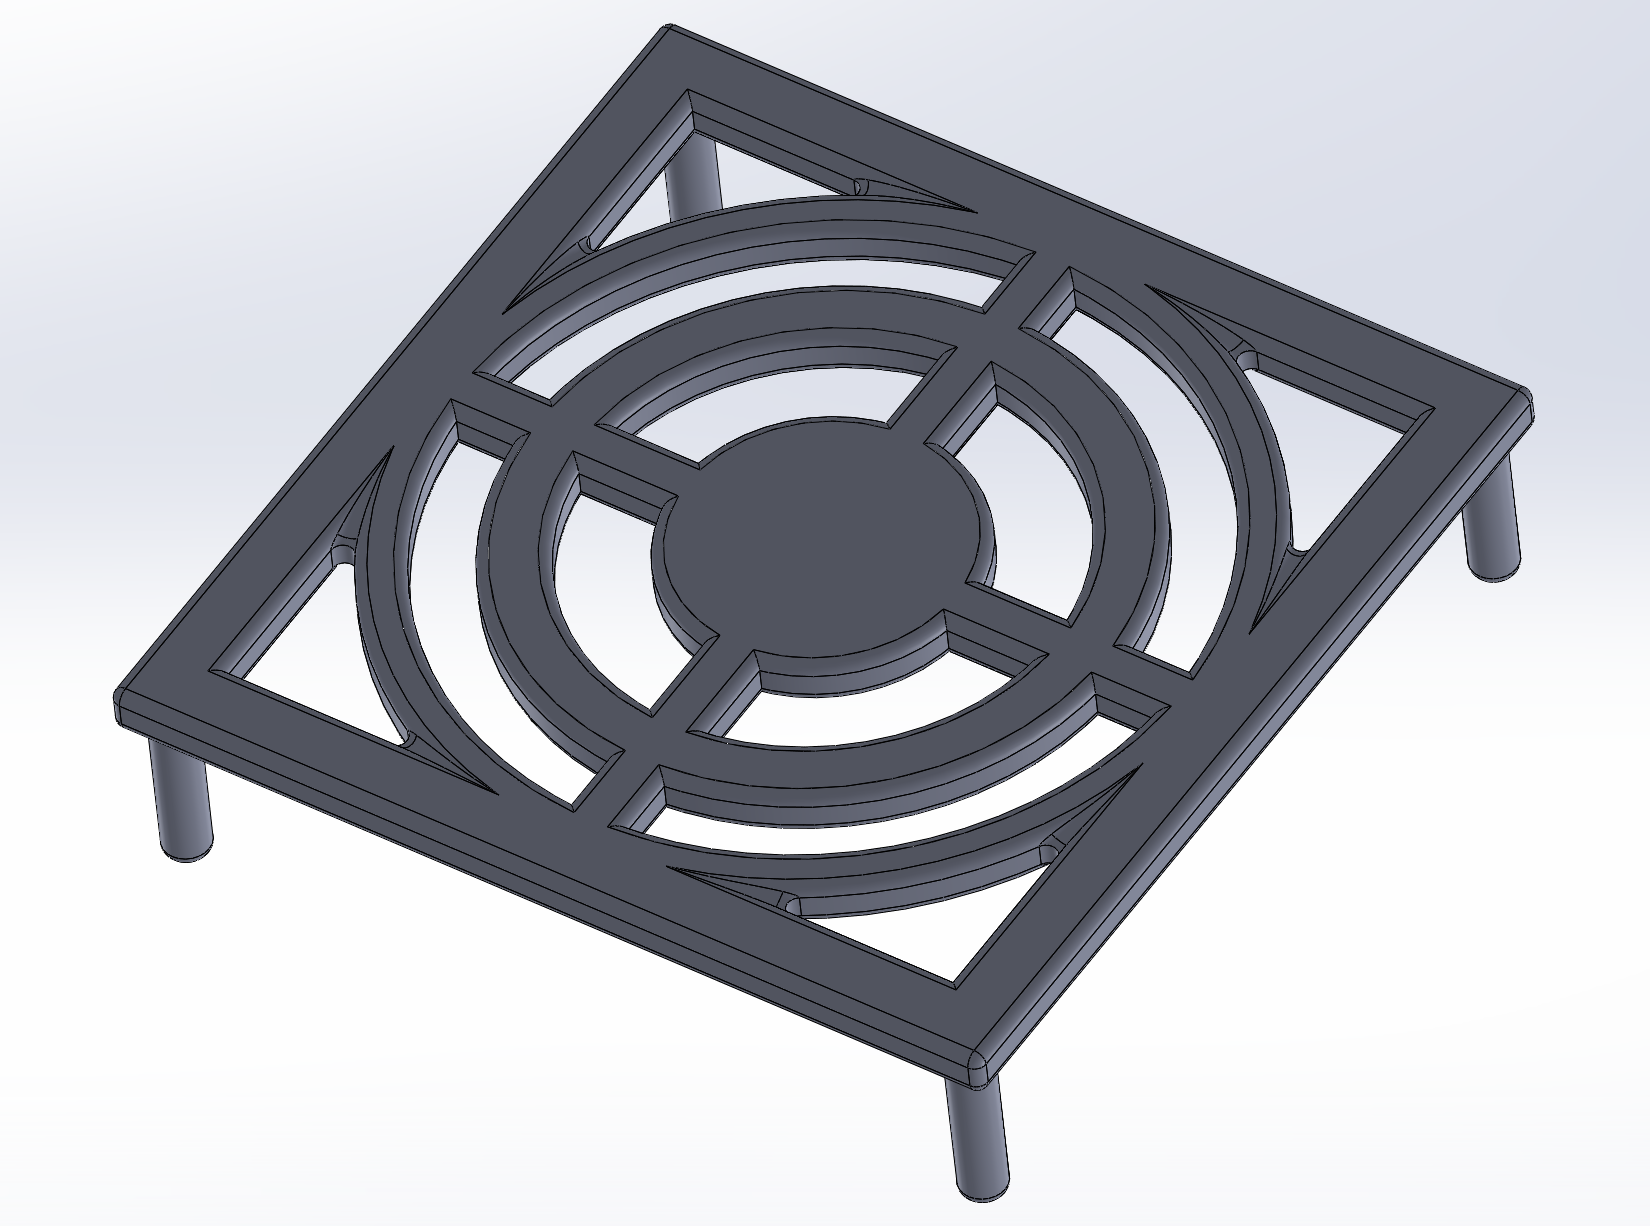
\includegraphics[width=12cm]{/3ddesign/fan.png}
\caption{A cover for the fan}
\label{fig::FAN}
\end{figure}

\subsection{Raspberry Pi Clamps}
The Raspberry Pi's used to be located in a small wooden box underneath the laptop.
They have now been moved to the front of WTR, in order to improve accessibility.
The mounts, as shown in figure \ref{fig::RPC}, have two holes in the bottom.
These fit a set of screws, and allow the mount to be attached to the wood plating.

\begin{figure}[H]
\centering
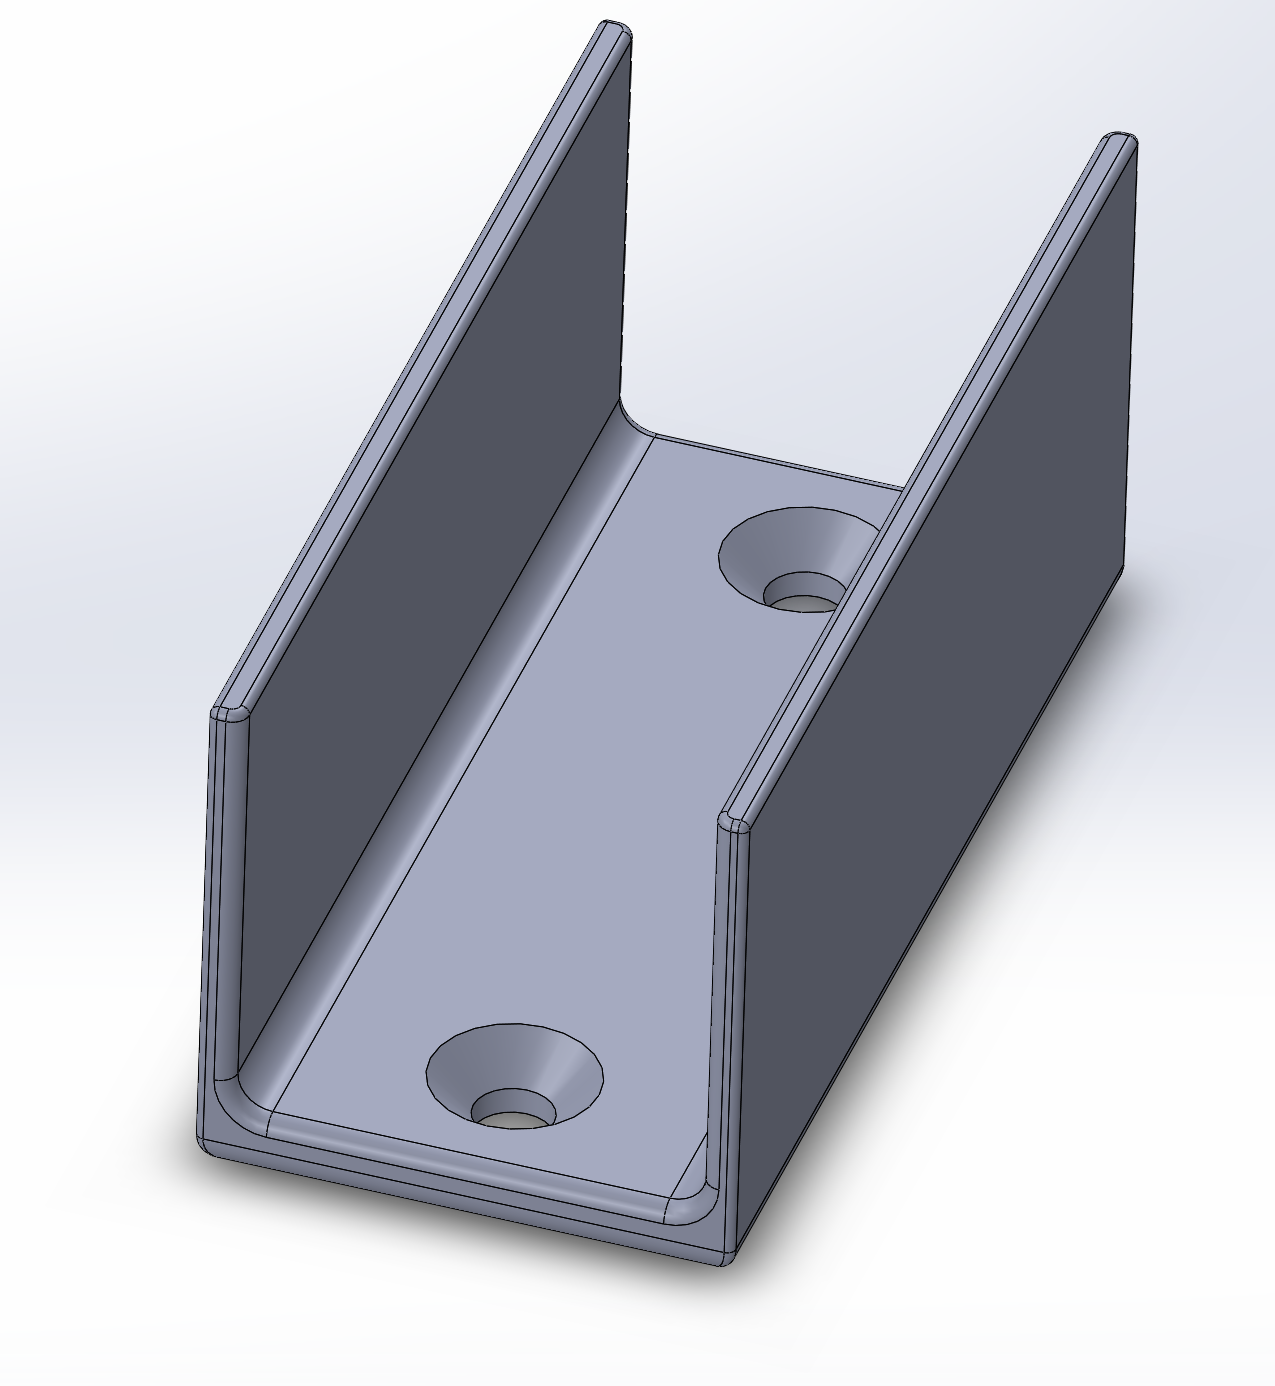
\includegraphics[width=12cm]{/3ddesign/RPC.png}
\caption{The Raspberry Pi mounts}
\label{fig::RPC}
\end{figure}


\newpage